\documentclass[11pt,aspectratio=169]{beamer}
 
\usetheme[sectionpage=none, subsectionpage=none, progressbar=none]{metropolis}           % Use metropolis theme
 
  \usepackage{outlines}
  \usepackage{caption}
  \usepackage{appendixnumberbeamer}
  \usepackage{booktabs}
  \usepackage{tcolorbox}
  \usepackage{tabularx}
  \usepackage[export]{adjustbox}[2011/08/13]
  \usepackage{bm}

\newcolumntype{R}{>{\raggedleft\arraybackslash}X} 

\newtheorem*{defn}{Def'n}

  
 \setbeamertemplate{footline}[frame number]{}

\setbeamertemplate{footline}{% 
  \hfill% 
  \usebeamercolor[fg]{page number in head/foot}% 
  \usebeamerfont{page number in head/foot}% 
  \insertframenumber%
  %\,/\,\inserttotalframenumber
  \kern1em\vskip2pt% 
}

\makeatletter
\setbeamertemplate{headline}{%
  \begin{beamercolorbox}[colsep=1.5pt]{upper separation line head}
  \end{beamercolorbox}
  \begin{beamercolorbox}{section in head/foot}
    \vskip2pt\insertnavigation{\paperwidth}\vskip2pt
  \end{beamercolorbox}%
  \begin{beamercolorbox}[colsep=1.5pt]{lower separation line head}
  \end{beamercolorbox}
}
\let\@@magyar@captionfix\relax % IMPORTANT: This is a workaround to fix a random eror with the 2018 installation
\makeatother

\usepackage{xcolor} 
\listfiles

\setbeamercolor{section in head/foot}{fg=normal text.bg, bg=structure.fg}

    \usepackage{smartdiagram}
    \usepackage{tikz}
\usetikzlibrary{shapes.geometric, arrows}
\tikzstyle{startstop} = [rectangle, rounded corners, minimum width=3cm, minimum height=1cm,text centered, draw=black, fill=red!30]
\tikzstyle{io} = [trapezium, trapezium left angle=70, trapezium right angle=110, minimum width=3cm, minimum height=1cm, text centered, draw=black, fill=blue!30]
\tikzstyle{process} = [rectangle, minimum width=3cm, minimum height=1cm, text centered, draw=black, fill=orange!30]
\tikzstyle{decision} = [diamond, minimum width=3cm, minimum height=1cm, text centered, draw=black, fill=green!30]

\title{Gov 2006: Formal Political Theory II \\
Section 6}
\date{\today}
\author{ \textbf{Sophie Hill}}


\begin{document}
  \maketitle
  
 %%%%%%%%%%%%%%%%%%%%%%%%%%%%%%%%%%%%%%%%%%
\begin{frame}{Reminder}

\begin{figure}
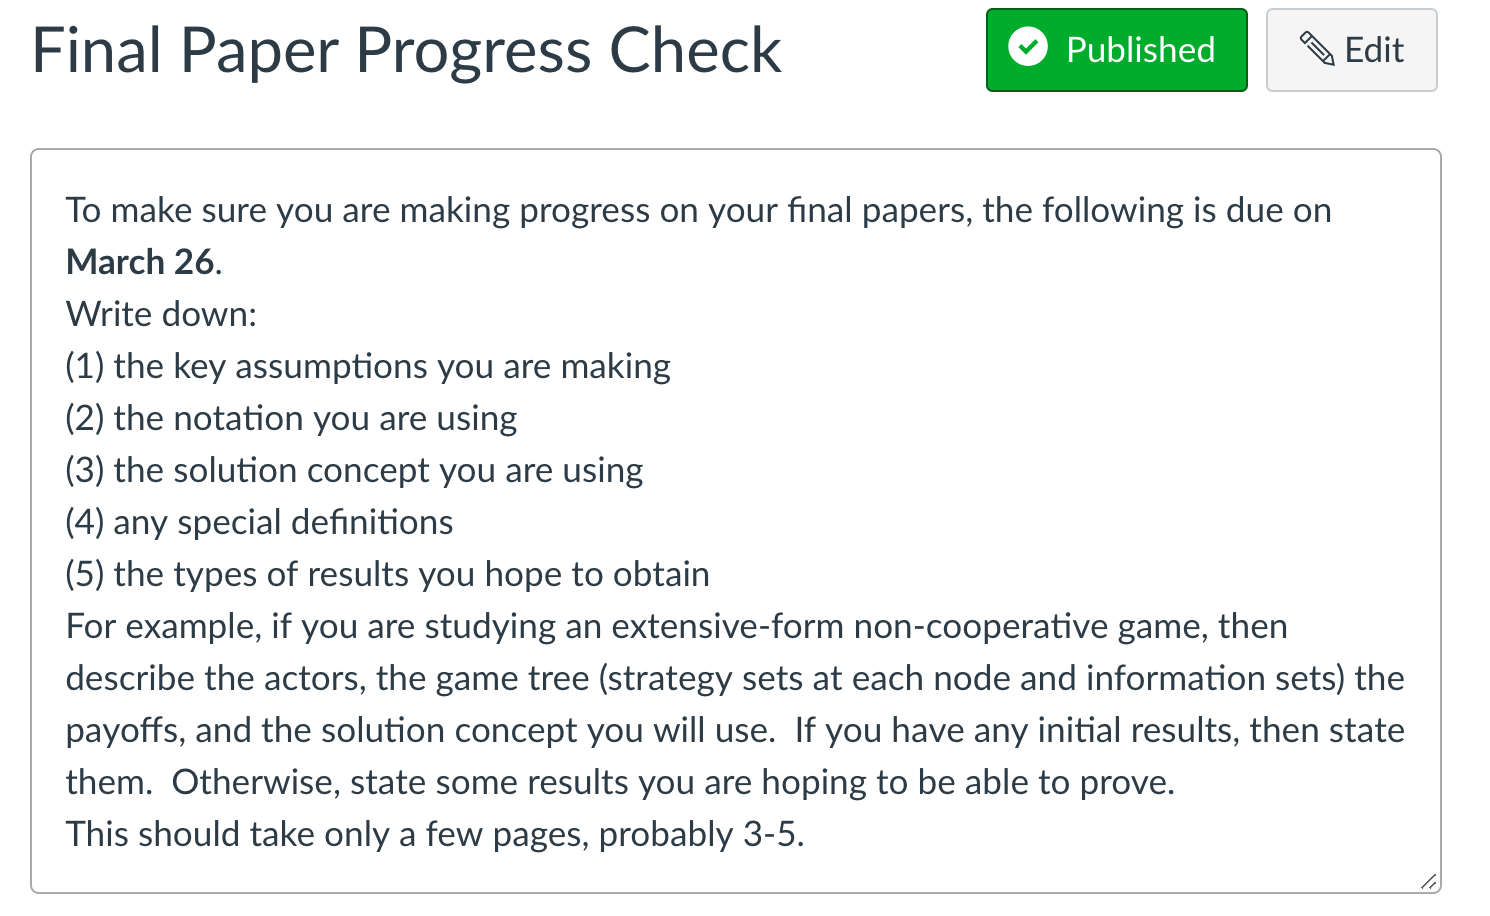
\includegraphics[width=0.8\textwidth]{canvas.png}
\end{figure}

\end{frame}

 %%%%%%%%%%%%%%%%%%%%%%%%%%%%%%%%%%%%%%%%%%
\begin{frame}{Reminder}

Section feedback form: \texttt{https://goo.gl/forms/ZYFgevfdeLNEpsnz2}

\vspace{2em}

My office hours are Mondays 2-4pm. However, I will be traveling Monday 25th March so I will hold extra OH later this week, or via slack.
\end{frame}

%%%%%%%%%%%%%%%%%%%%%%%%%%%%%%%%%%%%%%%%%%
\begin{frame}

\frametitle{Today}

\Large

Multidimensional electoral competition

\large
 
\begin{itemize}
\item Intermediate preferences
\item Recap main results from Plott \& McKelvey
\item Discussion: how should we interpret these results?
\end{itemize}


\end{frame}
%%%%%%%%%%%%%%%%%%%%%%%%%%%%%%%%%%%%%%%%%%
\begin{frame}{New definitions}

\begin{outline}
\1 The \textbf{top-cycle set} is the set of all $x$ such that for each $y \in X$ there exists a number $k$ and a sequence of alternatives $x_1, . . . , x_k$ with $x_1 = x, \, \,  x_k = y$, and $x_i T x_{i+1}$ for all $i = 1, . . . , k-1$.
\pause
\1 Problem: the top-cycle set is often very big!
\end{outline}

\end{frame}

%%%%%%%%%%%%%%%%%%%%%%%%%%%%%%%%%%%%%%%%%%
\begin{frame}{New definitions}

\begin{outline}
\1 Let $n(x, y)$ be the number of voters who (weakly) prefer $x$ to $y$. 
\1 Then \textbf{minmax set} is the set of policies whose maximal opposition is minimal. Formally: $minmax(X) = arg \, min_x max_{y \neq x} n(y, x)$.
\end{outline}

\end{frame}

%%%%%%%%%%%%%%%%%%%%%%%%%%%%%%%%%%%%%%%%%%
\begin{frame}{New definitions}

\begin{outline}
\1 The \textbf{uncovered set} is the set of alternatives each of which can defeat every other alternative in the space either directly or indirectly at one remove.
\1 Formally: $x \in X$ is \textit{covered} whenever there exists some other policy $y \in X$ such that $yPx$ and $\{ z: xPz \} \subseteq \{ z: yPz \}$
\end{outline}
\end{frame}

%%%%%%%%%%%%%%%%%%%%%%%%%%%%%%%%%%%%%%%%%%

\begin{frame}{Intermediate preferences}

\Large 

\begin{tcolorbox}
Voters have \textbf{intermediate preferences}, if their indirect utility
function $U(p;\alpha ^{i})$\ can be written as:
\begin{equation*}
U(p;\alpha ^{i})=J(p)+K(\alpha ^{i})H(p), 
\end{equation*}%
where $K(\alpha ^{i})$\ is monotonic in $\alpha ^{i},$\ for any $H(p)$\ and $%
J(p)$\ common to all voters.
\end{tcolorbox}

\pause

Intermediate preferences $\implies$ there is ``a single
source of disagreement among different individuals'' (PT, p.26)

\end{frame}
%%%%%%%%%%%%%%%%%%%%%%%%%%%%%%%%%%%%%%%%%%
\begin{frame}{Median Voter Theorem with Intermediate Preferences}

\Large 

\begin{tcolorbox}
\textbf{(Median Voter Theorem with Intermediate Preferences)}\emph{\ }
Suppose that voters vote sincerely and have intermediate preferences. Then a
Condorcet winner always exists and coincides with the bliss point of the
voter with the median value of $\alpha ^{i}$, $p(\alpha ^{m}).$
\end{tcolorbox}
\end{frame}

%%%%%%%%%%%%%%%%%%%%%%%%%%%%%%%%%%%%%%%%%%
\begin{frame}{Proof}

The proof is analogous to the proof of the median-voter theorem. Since $%
p(\alpha ^{m})$ is the maximum for agent $\alpha ^{m}$, we have that%
\begin{equation*}
U(p(\alpha ^{m});\alpha ^{m})=J(p(\alpha ^{m}))+K(\alpha ^{m})H(p(\alpha
^{m}))\geq U(p;\alpha ^{m})=J(p)+K(\alpha ^{m})H(p), 
\end{equation*}%
for all $p$. Therefore,%
\begin{eqnarray*}
K(\alpha ^{m}) &\lesseqqgtr &\frac{J(p(\alpha ^{m}))-J(p)}{H(p)-H(p(\alpha
^{m}))}\text{ as }H(p)\gtreqqless H(p(\alpha ^{m})), \\
\\
\text{for any }p &\neq &p(\alpha ^{m}).\text{ \ }
\end{eqnarray*}%
\end{frame}

%%%%%%%%%%%%%%%%%%%%%%%%%%%%%%%%%%%%%%%%%%
\begin{frame}{Proof (cont'd)}
Suppose that $H(p)<H(p(\alpha ^{m}))$ and $K(\alpha ^{i})$ is monotonically
increasing (the case of monotonically decreasing is analogous). Then $%
K(\alpha ^{i})\geq K(\alpha ^{m})$ for all $\alpha ^{i}>\alpha ^{m}$, and
these will all satisfy%
\begin{equation*}
K(\alpha ^{i})>\frac{J(p(\alpha ^{m}))-J(p)}{H(p)-H(p(\alpha ^{m}))} 
\end{equation*}%
and therefore%
\begin{equation*}
U(p(\alpha ^{m});\alpha ^{i})=J(p(\alpha ^{m}))+K(\alpha ^{i})H(p(\alpha
^{m}))\geq U(p;\alpha ^{i})=J(p)+K(\alpha ^{i})H(p), 
\end{equation*}%
so they will support $p(\alpha ^{m})$ against $p$. The other cases are
proved similarly. This shows that the policy $p(\alpha ^{m})$ always
collects at least half the votes against any alternative policy.

\end{frame}
%%%%%%%%%%%%%%%%%%%%%%%%%%%%%%%%%%%%%%%%%%
\begin{frame}{Plott (1967): Sufficient conditions for equilibrium}

\Large

Plott (1967) develops \alert{sufficient} (but not \alert{necessary}!) conditions for equilibrium in a multidimensional policy space with majority rule.

\vspace{1em}
\pause

Most famous is \textbf{pairwise symmetry} = all nonzero utility gradients at the equilibrium must be divisible into pairs that point in opposite directions.

\end{frame}

%%%%%%%%%%%%%%%%%%%%%%%%%%%%%%%%%%%%%%%%%%
\begin{frame}{Plott (1967): Sufficient conditions for equilibrium}

\begin{figure}
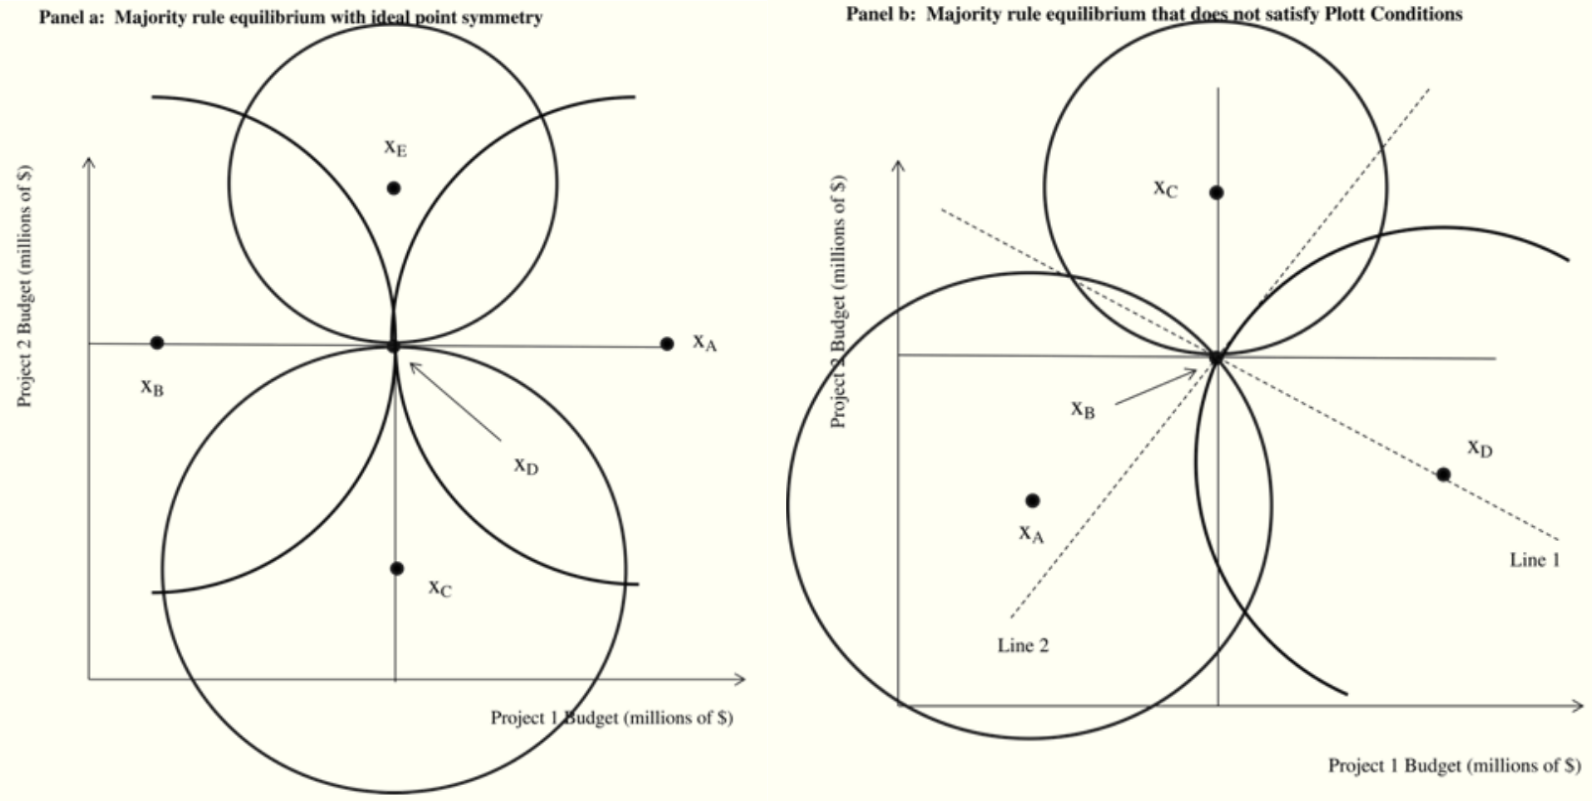
\includegraphics[width=1\textwidth]{plott.png}
\end{figure}

\end{frame}


%%%%%%%%%%%%%%%%%%%%%%%%%%%%%%%%%%%%%%%%%%
\begin{frame}{Plott (1967): Interpretation}

\Large

``The most important point is that there is certainly nothing inherent in utility theory which would assure the existence of an equilibrium. In fact, it would only be an accident (and a highly improbable one) if an equilibrium exists at all.'' \newline (Plott, 1967, pp.791-2)

\end{frame}
%%%%%%%%%%%%%%%%%%%%%%%%%%%%%%%%%%%%%%%%%%
\begin{frame}{McKelvey (1976): The ``chaos theorem''}

Assuming:
\begin{itemize}
\item A multidimensional policy space
\item at least 3 voters
\item sincere voting
\item Euclidean preferences
\item simple majority rule
\item Plott's symmetry condition doesn't hold
\end{itemize}

Then the cyclical top cycle set covers the whole
policy space. That is, the agenda setter can achieve \textit{any} policy outcome through a finite series of pairwise votes, regardless of the initial policy status quo. 



\end{frame}
%%%%%%%%%%%%%%%%%%%%%%%%%%%%%%%%%%%%%%%%%%
\begin{frame}{McKelvey (1976): The ``chaos theorem''}

\begin{figure}
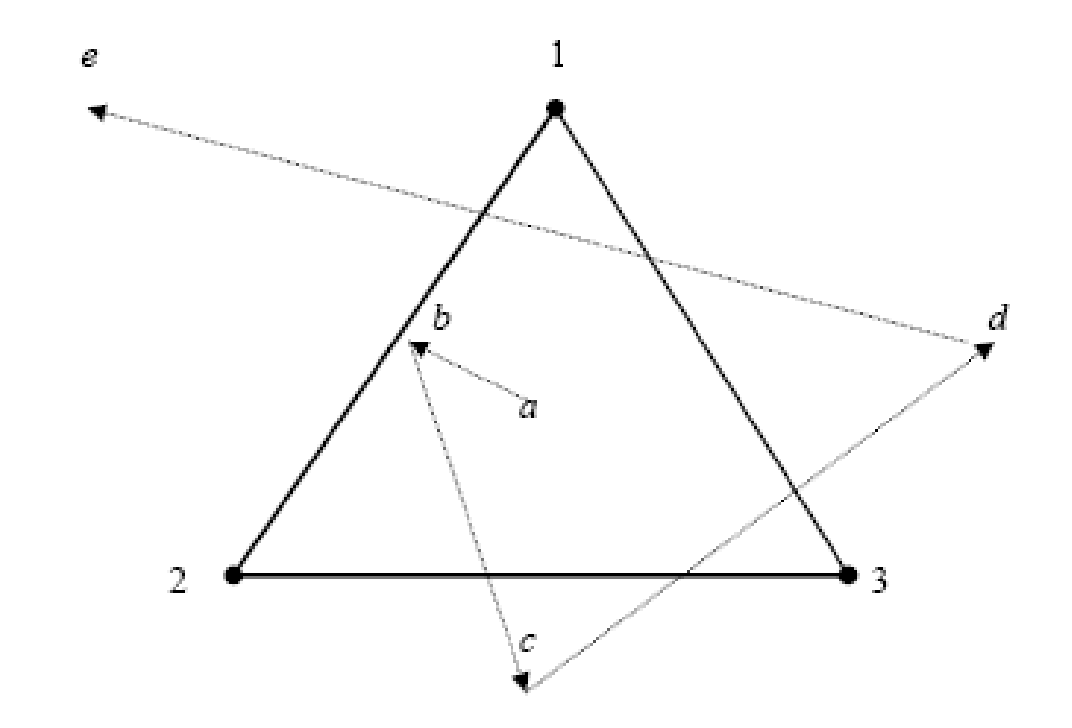
\includegraphics[width=0.75\textwidth]{mckelvey.png}
\end{figure}

\end{frame}
%%%%%%%%%%%%%%%%%%%%%%%%%%%%%%%%%%%%%%%%%%
\begin{frame}{Interpretation}

\Large

\begin{tcolorbox}
How should we interpret these results? Does McKelvey's ``Chaos Theorem'' imply actual chaos? 
\end{tcolorbox}

\end{frame}

%%%%%%%%%%%%%%%%%%%%%%%%%%%%%%%%%%%%%%%%%%
\begin{frame}{Response 1: Strategic behavior}

Recall that McKelvey's theorem assumes that voters are \alert{sincere}. The only strategic actor is (implicitly) the agenda-setter. Is this plausible?

\pause

\begin{tcolorbox}
\textbf{Example: The Powell Amendment*}
\newline A 1956 bill authorizing federal funding for schools is amended to require these schools to be racially desegregated. Some Republicans support the amendment strategically, knowing that Northern Democrats will not be able to justify voting against it -- as a result, the amended bill fails since both Republicans and Southern Democrats vote against.
\end{tcolorbox}

\pause 
\footnotesize *This example was popularized by Riker, though many scholars disagree with his interpretation! Nethertheless, it is a nice illustration of the logic...


\end{frame}
%%%%%%%%%%%%%%%%%%%%%%%%%%%%%%%%%%%%%%%%%%
\begin{frame}{Response 1: Strategic behavior}

\textbf{Definitions}
\newline A social choice function is \alert{strategyproof} if it is a dominant strategy for an individual to truthfully report her preferences. It is \alert{unanimous} if when everyone has the same preference order, the rule chooses that preference order.

\vspace{1.5em}
\pause

\begin{theorem}[Gibbard–Satterthwaite]
\vspace{0.2em}
Suppose there are at least three alternatives and that for each individual any strict ranking of these alternatives is permissible. Then the only unanimous, strategyproof social choice function is a dictatorship.
\end{theorem}


\end{frame}

%%%%%%%%%%%%%%%%%%%%%%%%%%%%%%%%%%%%%%%%%%

\begin{frame}{Response 2: Institutions matter!}

Recall that McKelvey's theorem also invokes a particular institutional set-up (pure majority rule with one fixed agenda-setter). What if we imposed a more realistic institutional structure?

\pause 
\textbf{Shepsle \& Weingast (1981)}: ``In our view, real-world legislative practices constrain the instability of PMR by restricting the domain and the content of legislative exchange.''

\pause
\textbf{BUT}: there is a famous objection to this line of reasoning...

\pause 
\textbf{Riker}: If certain institutions induce certain equilibria, then don't actors have preferences over institutions too (based on expected outcomes)? If so, the problem of instability returns!

\end{frame}

%%%%%%%%%%%%%%%%%%%%%%%%%%%%%%%%%%%%%%%%%%
\begin{frame}{Response 3: Uncertainty}

Probabilistic voting models introduce \alert{uncertainty}, which can either be viewed as random pre-election shocks to the candidates' favorability, or uncertainty from the candidates' perspective about the preferences of voters (or turnout). 

\vspace{2em}

For example, the model of \alert{Lindbeck \& Weibull (1987)} produces a Downsian (i.e. convergent) equilibrium, in which parties adopt identical platforms.


\end{frame}


\end{document}
